\chapter{Des quanta de corde ouverte aux tachyons et à la gravité}

\lectureoverview{Nous quantifions maintenant les modes normaux trouvés dans le cours précédent et nous demandons quels états de particules ils produisent. Chaque mode transverse est un oscillateur harmonique, mais sa normalisation est légèrement inhabituelle : exciter le mode \(n\) augmente l’énergie de front lumineux, et donc le niveau de masse au carré, de \(n\) unités. Le premier niveau excité de la corde ouverte se transforme exactement comme les deux polarisations transverses d’un vecteur sans masse. La cohérence relativiste impose donc une masse au carré négative pour l’état fondamental. Cet état est le tachyon de la corde bosonique, dont la véritable signification est celle d’un vide instable, et non d’une particule pratique se déplaçant plus vite que la lumière. Enfin, dès que les cordes interagissent, les processus de jonction et de scission rendent inévitables les cordes fermées ; l’excitation de plus basse énergie d’une corde fermée sera le graviton.}

\section{L’oscillateur caché dans chaque mode de la corde}

Pour une coordonnée transverse \(X\), le \(n\)e mode normal non nul a pour énergie et lagrangien

\begin{align}
  E_n
  &=
  \frac14\dot X_n^{\,2}
  +\frac{n^2}{4}X_n^2,
  \label{eq:l03-mode-energy}\\
  L_n
  &=
  \frac14\dot X_n^{\,2}
  -\frac{n^2}{4}X_n^2.
  \label{eq:l03-mode-lagrangian}
\end{align}

Les facteurs \(1/4\) ne sont pas une erreur. Ils reflètent la normalisation choisie lorsque l’action de la corde a été réduite à des modes de Fourier indépendants. La première étape de la construction du hamiltonien consiste donc à calculer l’impulsion canonique,

\begin{equation}
  p_n=\frac{\partial L_n}{\partial\dot X_n}
     =\frac12\dot X_n,
  \qquad
  \dot X_n=2p_n.
  \label{eq:l03-canonical-momentum}
\end{equation}

La transformation de Legendre donne

\begin{equation}
  H_n=p_n\dot X_n-L_n
     =p_n^2+\frac{n^2}{4}X_n^2.
  \label{eq:l03-mode-hamiltonian}
\end{equation}

\begin{figure}[H]\centering
  \includegraphics[width=0.82\textwidth]{lecture_03_figure_01.png}\caption{Énergie du mode, lagrangien, impulsion canonique et hamiltonien dans la normalisation héritée de la corde ouverte.}\lectureframe{00:05:40}\label{fig:l03-mode-hamiltonian-board}\end{figure}

Pour factoriser \(H_n\), combinons \(X_n\) et \(p_n\) comme suit :

\begin{equation}
  \frac{nX_n}{2}\pm i p_n.
\end{equation}

Classiquement, les deux facteurs commuteraient, mais en mécanique quantique,

\begin{equation}
  [X_n,p_m]=i\delta_{nm}
  \label{eq:l03-canonical-commutator}
\end{equation}

dans les unités où \(\hbar=1\). Les termes croisés ne s’annulent pas sans laisser de trace. Pour un mode donné,

\begin{align}
  \left[\frac{nX_n}{2}+ip_n,
        \frac{nX_n}{2}-ip_n\right]
  &=n,
  \label{eq:l03-unscaled-commutator}\\
  \left(\frac{nX_n}{2}-ip_n\right)
  \left(\frac{nX_n}{2}+ip_n\right)
  &=H_n-\frac n2.
  \label{eq:l03-factorized-hamiltonian}
\end{align}

\begin{figure}[H]\centering
  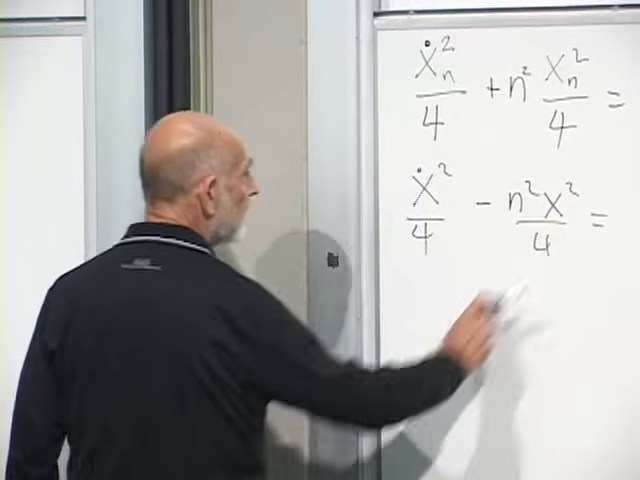
\includegraphics[width=0.82\textwidth]{lecture_03_figure_02.png}\caption{Le calcul au tableau, où le commutateur canonique fournit le facteur \(n\).}\lectureframe{00:10:30}\label{fig:l03-commutator-board}\end{figure}

Le facteur \(n\) nous indique comment normaliser les opérateurs d’échelle :

\begin{align}
  a_n
  &\equiv
  \frac{\sqrt n}{2}X_n+\frac{i}{\sqrt n}p_n,
  \label{eq:l03-annihilator}\\
  a_n^\dagger
  &\equiv
  \frac{\sqrt n}{2}X_n-\frac{i}{\sqrt n}p_n.
  \label{eq:l03-creator}
\end{align}

Ils vérifient

\begin{equation}
  [a_n,a_m^\dagger]=\delta_{nm},
  \qquad
  H_n=n\left(a_n^\dagger a_n+\frac12\right).
  \label{eq:l03-oscillator-algebra}
\end{equation}

Ainsi, \(a_n^\dagger\) ajoute un quantum au \(n\)e oscillateur, mais ce quantum porte une énergie de mode de \(n\) unités. L’espacement familier de l’oscillateur n’a pas disparu ; sa fréquence est \(\omega_n=n\).

\begin{figure}[H]\centering
  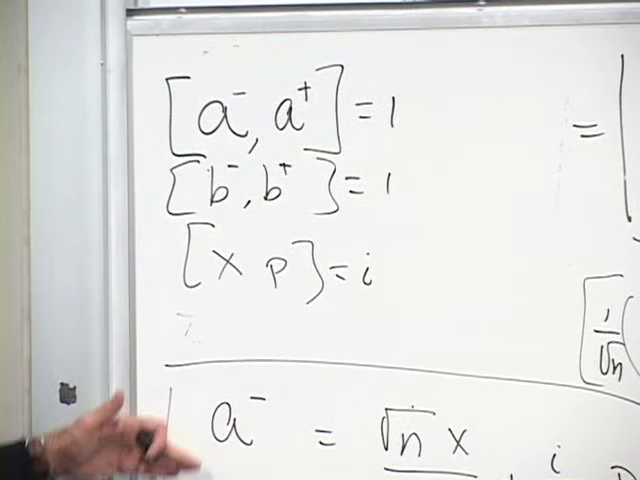
\includegraphics[width=0.82\textwidth]{lecture_03_figure_03.png}\caption{Opérateurs d’annihilation et de création normalisés pour le \(n\)e oscillateur de la corde.}\lectureframe{00:12:00}\label{fig:l03-ladder-board}\end{figure}

\subsection{Deux tours transverses}

Dans un espace-temps à quatre dimensions, une corde portant une très grande quantité de mouvement selon l’axe \(z\) a deux coordonnées transverses, \(X\) et \(Y\). Il nous faut donc deux tours d’oscillateurs indépendants. Notons \(a_n,a_n^\dagger\) les opérateurs agissant sur les modes \(X\) et \(b_n,b_n^\dagger\) ceux qui agissent sur les modes \(Y\). Résoudre \eqref{eq:l03-annihilator}--\eqref{eq:l03-creator} par rapport aux coordonnées donne

\begin{equation}
  X_n=\frac{a_n+a_n^\dagger}{\sqrt n},
  \qquad
  Y_n=\frac{b_n+b_n^\dagger}{\sqrt n}.
  \label{eq:l03-mode-coordinates}
\end{equation}

\begin{figure}[H]\centering
  \includegraphics[width=0.78\textwidth]{lecture_03_figure_04.png}\caption{Résolution de la coordonnée d’un mode en fonction de ses opérateurs de création et d’annihilation.}\lectureframe{00:17:05}\label{fig:l03-coordinate-operator-board}\end{figure}

Les coordonnées de la corde ouverte ont été développées en modes de Neumann,

\begin{align}
  X(\sigma,\tau)
  &=X_{\rm cm}(\tau)
    +\sum_{n=1}^{\infty}X_n(\tau)\cos(n\sigma),
  \label{eq:l03-X-fourier}\\
  Y(\sigma,\tau)
  &=Y_{\rm cm}(\tau)
    +\sum_{n=1}^{\infty}Y_n(\tau)\cos(n\sigma).
  \label{eq:l03-Y-fourier}
\end{align}

Les cosinus apparaissent parce que les pentes aux extrémités s’annulent. En substituant \eqref{eq:l03-mode-coordinates}, on transforme la corde elle-même en opérateur :

\begin{align}
  X(\sigma,\tau)
  &=X_{\rm cm}(\tau)
    +\sum_{n=1}^{\infty}
      \frac{a_n(\tau)+a_n^\dagger(\tau)}{\sqrt n}
      \cos(n\sigma),
  \label{eq:l03-X-operator}\\
  Y(\sigma,\tau)
  &=Y_{\rm cm}(\tau)
    +\sum_{n=1}^{\infty}
      \frac{b_n(\tau)+b_n^\dagger(\tau)}{\sqrt n}
      \cos(n\sigma).
  \label{eq:l03-Y-operator}
\end{align}

\begin{figure}[H]\centering
  \begin{minipage}[t]{0.48\textwidth}\centering
    \includegraphics[width=\textwidth]{lecture_03_figure_05.png}\par\smallskip\footnotesize (a) Développements en modes des coordonnées. \end{minipage}\hfill
  \begin{minipage}[t]{0.48\textwidth}\centering
    \includegraphics[width=\textwidth]{lecture_03_figure_06.png}\par\smallskip\footnotesize (b) Opérateurs d’échelle substitués dans les coordonnées de la corde.\end{minipage}\caption{La forme de la corde ouverte quantique est assemblée à partir de tous ses opérateurs d’oscillateurs transverses.}\lectureframe{00:20:35 and 00:21:05}\label{fig:l03-string-coordinate-board}\end{figure}

\begin{classroomqa}\audiencequestion{\(X_n\) est-il également fonction de \(\sigma\) ?\lecturetimestamp{00:21:48}}\lecturerresponse{Non. La dépendance en \(\sigma\) se trouve entièrement dans \(\cos(n\sigma)\). Le coefficient \(X_n\) est l’amplitude, dépendante du temps, de ce profil spatial ; ainsi, \(X_n=X_n(\tau)\).}\end{classroomqa}

\begin{classroomqa}\audiencequestion{Pourquoi les opérateurs appelés opérateurs de montée et de descente semblent-ils avoir leurs signes inversés ?\lecturetimestamp{00:23:13}}\lecturerresponse{Le signe visible de \(ip_n\) ne détermine pas le nom de l’opérateur. Calculons le commutateur avec le hamiltonien. L’opérateur qui vérifie \([H_n,a_n^\dagger]=n a_n^\dagger\) augmente l’énergie ; celui qui vérifie \([H_n,a_n]=-n a_n\) la diminue.}\end{classroomqa}

Les deux tours transverses constituent une représentation pédagogique en quatre dimensions. Une corde bosonique quantifiée de façon cohérente possède vingt-six dimensions d’espace-temps ; elle a donc vingt-quatre familles d’oscillateurs transverses, au lieu de deux. Le raisonnement qui suit reste le même : le nombre d’états du premier niveau doit correspondre au nombre de polarisations physiques d’un vecteur sans masse dans la même dimension.

\section{Spin massif et hélicité sans masse}

Avant d’attribuer un spin aux états de la corde, il faut établir une distinction nette. Une particule massive de spin \(J\) possède \(2J+1\) états de spin,

\begin{equation}
  m_J=-J,-J+1,\ldots,J-1,J.
  \label{eq:l03-massive-spin-multiplet}
\end{equation}

Par exemple, une particule massive de spin un possède trois polarisations et une particule massive de spin deux en possède cinq. On comprend pourquoi en se plaçant dans le référentiel au repos. Toutes les rotations spatiales y sont possibles. On fait tourner l’axe de spin, puis on effectue un boost en retour ; les \(2J+1\) composantes appartiennent alors toutes à la même particule relativiste.

Une particule sans masse n’a pas de référentiel au repos. Son étiquette de spin invariante est l’hélicité, c’est-à-dire le moment cinétique selon sa direction de mouvement. Un photon n’a que les hélicités \(h=+1\) et \(h=-1\) ; un graviton n’a que \(h=+2\) et \(h=-2\). Un scalaire n’a qu’un état \(h=0\). Le cours utilise la symétrie par réflexion pour associer les deux hélicités. Dans une théorie chirale, une représentation irréductible sans masse peut ne porter qu’une seule hélicité ; l’association des deux est donc une affirmation de symétrie supplémentaire, et non une conséquence de la seule absence de masse.\editorialnote{La classification moderne par le groupe petit admet des représentations sans masse à une seule hélicité. La parité ou un contenu de champs approprié, complété par CPT, fournit l’hélicité opposée dans les exemples familiers du photon et du graviton.}

\begin{figure}[H]\centering
  \begin{minipage}[t]{0.45\textwidth}\centering
    \includegraphics[width=\textwidth]{lecture_03_figure_07.png}\par\smallskip\footnotesize (a) Le décompte des états de spin commencé au tableau. \end{minipage}\hfill
  \begin{minipage}[t]{0.5\textwidth}\centering
    \begin{adjustbox}{max width=\linewidth}\begin{tabular}{@{}ccc@{}}\toprule
      Spin & États massifs & Hélicités sans masse \\\midrule
      \(0\)&\(1\)&\(0\)\\\(1\)&\(3\)&\(+1,-1\)\\\(2\)&\(5\)&\(+2,-2\)\\\bottomrule
    \end{tabular}\end{adjustbox}\end{minipage}\caption{La masse élimine le référentiel au repos et, avec lui, les projections de spin intermédiaires.}\lectureframe{00:27:40}\label{fig:l03-spin-count}\end{figure}

\subsection{Polarisation linéaire et circulaire du photon}

Considérons un photon qui se déplace selon \(z\). Ses deux polarisations linéaires transverses sont \(\ket{x}\) et \(\ket{y}\). Elles ne sont pas des états propres de l’hélicité. Les états circulaires sont

\begin{align}
  \ket{R}
  &=\frac{1}{\sqrt2}\left(\ket{x}+i\ket{y}\right),
  \label{eq:l03-right-circular}\\
  \ket{L}
  &=\frac{1}{\sqrt2}\left(\ket{x}-i\ket{y}\right),
  \label{eq:l03-left-circular}
\end{align}

avec les hélicités \(+1\) et \(-1\), selon la convention adoptée pour nommer les polarisations droite et gauche. Un photon polarisé linéairement est une superposition de ces deux résultats possibles. Son hélicité moyenne peut être nulle, mais une mesure de l’hélicité ne donne jamais un photon de spin nul. De même,

\begin{equation}
  \frac{1}{\sqrt2}\left(\ket{x}+\ket{y}\right)
\end{equation}

correspond simplement à une polarisation linéaire à quarante-cinq degrés.

\begin{figure}[H]\centering
  \begin{minipage}[t]{0.48\textwidth}\centering
    \includegraphics[width=\textwidth]{lecture_03_figure_08.png}\par\smallskip\footnotesize (a) États de polarisation circulaire au tableau. \end{minipage}\hfill
  \begin{minipage}[t]{0.48\textwidth}\centering
    \begin{adjustbox}{max width=\linewidth}\begin{tikzpicture}[>=Latex,scale=0.9]
      \draw[->,thick] (0,0) -- (3.4,0) node[right] {\(z\)};
      \draw[->,blue!70!black,thick] (0,0) -- (0,2.0)
        node[above] {\(x\)};
      \draw[->,orange!85!black,thick] (0,0) -- (-1.4,-1.2)
        node[below left] {\(y\)};
      \draw[red!70!black,thick,->]
        plot[domain=0:320,samples=80]
        ({1.0*cos(\x)},{0.58*sin(\x)+0.4});
      \node[red!70!black] at (1.55,1.25) {circular};
    \end{tikzpicture}\end{adjustbox}\end{minipage}\caption{Une base transverse est fournie par la polarisation linéaire ; les combinaisons circulaires diagonalisent l’hélicité.}\lectureframe{00:37:45}\label{fig:l03-polarization}\end{figure}

\begin{classroomqa}\audiencequestion{Est-ce analogue à la séparation des états de spin dans une expérience de Stern--Gerlach ?\lecturetimestamp{00:37:40}}\lecturerresponse{L’idée de superposition quantique est la même, mais pour le photon, le langage direct est celui de la polarisation. Une mesure de la polarisation circulaire distingue les deux hélicités ; le faisceau ne contient pas de photon longitudinal de spin nul.}\end{classroomqa}

Le graviton reprend le même schéma avec le spin deux. Pour tenir compte des spins, on peut écrire schématiquement

\begin{equation}
  \ket{+2}\sim\ket{+1}\otimes\ket{+1},
  \qquad
  \ket{-2}\sim\ket{-1}\otimes\ket{-1}.
  \label{eq:l03-graviton-helicity}
\end{equation}

Cela ne signifie pas qu’un graviton est littéralement constitué de deux photons. Cela signifie que deux hélicités égales s’additionnent pour donner l’hélicité correcte de spin deux.

\begin{classroomqa}\audiencequestion{L’analogie avec deux photons s’étend-elle à d’autres nombres quantiques ?\lecturetimestamp{00:41:05}}\lecturerresponse{Pas comme modèle de constituants. Il existe des formules puissantes dans lesquelles les amplitudes gravitationnelles ressemblent à des produits, ou à des carrés``'', d’amplitudes de théorie de jauge, mais le graviton reste une particule à part entière. Ici, l’analogie est surtout fiable comme énoncé sur l’hélicité.\editorialnote{Les relations modernes de Kawai--Lewellen--Tye et de double copie précisent l’énoncé sur les amplitudes dans certaines théories ; elles ne font pas du graviton un état lié de deux photons.}}\end{classroomqa}

\begin{classroomqa}\audiencequestion{Un photon peut avoir n’importe quelle quantité de mouvement ; son spectre n’est-il donc pas continu, au lieu d’être discret comme l’exige celui d’une particule ?\lecturetimestamp{00:42:17}}\lecturerresponse{La variable continue est la quantité de mouvement du centre de masse. Fixons cette quantité de mouvement et examinons la masse invariante interne. Une particule est identifiée par un niveau de masse discret ; la variation de sa quantité de mouvement globale produit ensuite la relation de dispersion continue habituelle.}\end{classroomqa}

\section{Les niveaux les plus bas de la corde ouverte}

Nous pouvons maintenant revenir à la corde. Dans la description à grande quantité de mouvement, l’énergie interne finie de front lumineux est proportionnelle à la masse invariante au carré. En omettant le facteur global correspondant à l’échelle de la corde, écrivons le spectre sous la forme

\begin{equation}
  \begin{aligned}
    M^2
    &=m_0^2
      +\sum_{n=1}^{\infty}n
       \left(N_n^{(a)}+N_n^{(b)}\right),\\
    N_n^{(a)}&=a_n^\dagger a_n,
    \qquad
    N_n^{(b)}=b_n^\dagger b_n.
  \end{aligned}
  \label{eq:l03-open-spectrum}
\end{equation}

L’état fondamental de l’oscillateur vérifie

\begin{equation}
  a_n\ket{0}=0,
  \qquad
  b_n\ket{0}=0,
  \qquad n=1,2,\ldots .
  \label{eq:l03-ground-annihilation}
\end{equation}

Ce n’est pas une absence de corde. C’est l’état quantique le moins excité de la corde, dont les coordonnées fluctuent toujours. Notons sa masse au carré \(m_0^2\), qu’il reste à déterminer.

\begin{figure}[H]\centering
  \includegraphics[width=0.78\textwidth]{lecture_03_figure_09.png}\caption{L’état fondamental de la corde ouverte et les conditions d’annihilation qui le définissent.}\lectureframe{00:45:20}\label{fig:l03-ground-state-board}\end{figure}

Les excitations les moins coûteuses font intervenir les opérateurs de création \(n=1\) :

\begin{equation}
  a_1^\dagger\ket{0},
  \qquad
  b_1^\dagger\ket{0},
  \qquad
  M^2=m_0^2+1.
  \label{eq:l03-first-level}
\end{equation}

\begin{figure}[H]\centering
  \includegraphics[width=0.78\textwidth]{lecture_03_figure_10.png}\caption{L’un des deux états dégénérés du premier niveau, avec l’incrément de masse au carré inscrit au tableau.}\lectureframe{00:49:25}\label{fig:l03-first-level-board}\end{figure}

Le mot ``un'' dans l’eqref{eq:l03-first-level} ne désigne pas un joule, un électronvolt ni une masse de Planck. Nous avons omis l’échelle dimensionnée de la corde. Pour l’instant, il signifie un échelon dans la tour des masses au carré de l’oscillateur ; les unités manquantes seront rétablies au cours suivant.

Toute combinaison linéaire des deux états dégénérés est également un état de ce niveau. En particulier,

\begin{equation}
  \frac{1}{\sqrt2}
  \left(a_1^\dagger\pm i b_1^\dagger\right)\ket{0}
  \label{eq:l03-string-circular-states}
\end{equation}

est l’analogue, pour la corde, de la polarisation circulaire. Sous une rotation dans le plan \(x\)-\(y\), \(a_1^\dagger\) et \(b_1^\dagger\) se transforment comme les deux composantes d’un vecteur transverse. Les combinaisons de \eqref{eq:l03-string-circular-states} ont donc les hélicités \(+1\) et \(-1\).

\begin{figure}[H]\centering
  \includegraphics[width=0.82\textwidth]{lecture_03_figure_11.png}\caption{Conditions de l’état fondamental, deux excitations du premier niveau et leurs combinaisons circulaires, réunies au tableau.}\lectureframe{00:56:00}\label{fig:l03-level-structure-board}\end{figure}

Il n’existe pas de troisième état dégénéré qui puisse servir de polarisation longitudinale. Si ces deux états avaient une masse non nulle, une particule relativiste de spin un exigerait trois polarisations. Avec exactement deux polarisations, l’état doit donc être sans masse. Ainsi,

\begin{equation}
  m_0^2+1=0,
  \qquad
  m_0^2=-1.
  \label{eq:l03-intercept-condition}
\end{equation}

Le premier niveau ressemble à celui du photon : c’est un état de vecteur de jauge sans masse. Il ne s’agit pas nécessairement du photon de l’électromagnétisme ; son identité de jauge éventuelle dépend du modèle de corde. L’état fondamental qui lui est inférieur a une masse au carré négative. C’est le tachyon de la corde bosonique ouverte.\editorialnote{Dans la corde bosonique critique complète, l’intercept de l’ordre normal et l’algèbre de Lorentz sont liés à \(D=26\). Le calcul du cours avec deux directions transverses est la projection en quatre dimensions du même argument de dénombrement des états : les états d’oscillateur du premier niveau, au nombre de \(D-2\), correspondent aux polarisations physiques d’un vecteur sans masse, au nombre de \(D-2\).}

\begin{classroomqa}\audiencequestion{Pourquoi faut-il s’intéresser au fait que \(m_0^2\) est négative ?\lecturetimestamp{00:56:35}}\lecturerresponse{Parce que la masse au carré est la courbure du potentiel quadratique du champ autour de l’état que nous avons appelé le vide. Une courbure négative signifie que cette configuration n’est pas un état fondamental stable. Le calcul suivant rend cette affirmation précise.}\end{classroomqa}

\section{Ce que signifie réellement un tachyon}

Le nom ``tachyon'' suggère d’abord une idée trompeuse. Partons de la relation de dispersion relativiste avec \(c=1\),

\begin{equation}
  E(p)=\sqrt{p^2+m^2}.
  \label{eq:l03-relativistic-dispersion}
\end{equation}

Pour un paquet d’ondes, la vitesse de groupe est

\begin{equation}
  v_g=\frac{dE}{dp}.
  \label{eq:l03-group-velocity}
\end{equation}

On retrouve ainsi des cas familiers :

\begin{align}
  E_{\rm nr}(p)&=\frac{p^2}{2m},
  &v_g&=\frac{p}{m},
  \label{eq:l03-nr-group-velocity}\\
  E_\gamma(p)&=|p|,
  &|v_g|&=1,
  \label{eq:l03-photon-group-velocity}\\
  E_m(p)&=\sqrt{p^2+m^2},
  &|v_g|&=\frac{|p|}{\sqrt{p^2+m^2}}<1.
  \label{eq:l03-massive-group-velocity}
\end{align}

\begin{figure}[H]\centering
  \begin{minipage}[t]{0.48\textwidth}\centering
    \includegraphics[width=\textwidth]{lecture_03_figure_12.png}\par\smallskip\footnotesize (a) Vitesse de groupe non relativiste. \end{minipage}\hfill
  \begin{minipage}[t]{0.48\textwidth}\centering
    \includegraphics[width=\textwidth]{lecture_03_figure_13.png}\par\smallskip\footnotesize (b) Relation de dispersion relativiste et sa dérivée.\end{minipage}\caption{Lire la vitesse de propagation sur la pente de \(E(p)\).}\lectureframe{01:01:50 and 01:03:15}\label{fig:l03-group-velocity-board}\end{figure}

Si \(m^2=-\mu^2\), l’expression formelle devient

\begin{equation}
  E(p)=\sqrt{p^2-\mu^2},
  \qquad
  v_g=\frac{p}{\sqrt{p^2-\mu^2}},
  \label{eq:l03-formal-tachyon-dispersion}
\end{equation}

qui vérifie \(|v_g|>1\) chaque fois que la racine carrée est réelle. Mais ce n’est pas la bonne interprétation physique de l’état fondamental de la corde bosonique. Le problème apparaît déjà à faible quantité de mouvement, où la fréquence est imaginaire.

\subsection{Courbure négative du potentiel du champ}

Considérons un champ scalaire réel en une dimension spatiale,

\begin{equation}
  \left(\partial_t^2-\partial_x^2+m^2\right)\phi=0.
  \label{eq:l03-klein-gordon}
\end{equation}

Pour une onde plane \(\phi\propto e^{-i\omega t+ikx}\),

\begin{equation}
  \omega^2=k^2+m^2.
  \label{eq:l03-kg-dispersion}
\end{equation}

\begin{figure}[H]\centering
  \includegraphics[width=0.82\textwidth]{lecture_03_figure_14.png}\caption{L’équation de Klein--Gordon utilisée pour mettre en évidence l’instabilité associée à une masse au carré négative.}\lectureframe{01:06:40}\label{fig:l03-klein-gordon-board}\end{figure}

L’énergie quadratique conservée est

\begin{equation}
  \mathcal E
  =\frac12\int dx\,
  \left[
    \dot\phi^{\,2}
    +(\partial_x\phi)^2
    +m^2\phi^2
  \right].
  \label{eq:l03-field-energy}
\end{equation}

\begin{figure}[H]\centering
  \includegraphics[width=0.82\textwidth]{lecture_03_figure_15.png}\caption{Énergie du champ scalaire, dont le terme de masse donne la courbure locale du potentiel.}\lectureframe{01:08:10}\label{fig:l03-field-energy-board}\end{figure}

Pour \(m^2>0\), le potentiel local \(V(\phi)=\tfrac12m^2\phi^2\) a la forme d’une cuvette. La configuration \(\phi=0\) se trouve au fond. Pour \(m^2=-\mu^2\), le même point est au sommet d’une cuvette inversée. L’équation \eqref{eq:l03-kg-dispersion} devient

\begin{equation}
  \omega^2=k^2-\mu^2.
  \label{eq:l03-tachyonic-modes}
\end{equation}

Les modes tels que \(k^2<\mu^2\) ont

\begin{equation}
  \omega=\pm i\sqrt{\mu^2-k^2},
  \qquad
  \phi_k(t)\propto
  e^{\pm\sqrt{\mu^2-k^2}\,t}.
  \label{eq:l03-growing-mode}
\end{equation}

Une branche croît exponentiellement. Le prétendu vide est donc instable : une perturbation de grande longueur d’onde, aussi petite soit-elle, éloigne le champ de \(\phi=0\). Voilà ce que signifie la présence d’un tachyon dans le spectre.

\subsection{La chaîne de pendules en équilibre instable}

Une rangée de pendules couplés rend cette distinction visible. Plaçons tous les pendules à la verticale, en équilibre inversé. La configuration uniforme existe, mais elle est en équilibre au maximum de l’énergie potentielle. On donne une légère impulsion à un pendule ; il tombe et entraîne ses voisins. Un front de chute se propage le long de la chaîne à la vitesse de signal finie imposée par les couplages.

\begin{figure}[H]\centering
  \begin{minipage}[t]{0.48\textwidth}\centering
    \includegraphics[width=\textwidth]{lecture_03_figure_16.png}\par\smallskip\footnotesize (a) Le modèle de pendules couplés en équilibre inversé, au tableau. \end{minipage}\hfill
  \begin{minipage}[t]{0.48\textwidth}\centering
    \begin{adjustbox}{max width=\linewidth}\begin{tikzpicture}[>=Latex,scale=0.78]
      \draw[thick] (-0.3,0) -- (6.3,0);
      \foreach \x/\a in {0/0,1/0,2/8,3/28,4/55,5/72,6/78}{
        \fill (\x,0) circle (0.06);
        \draw[thick] (\x,0) -- ++({90-\a}:1.25);
        \fill[blue!65!black]
          ($(\x,0)+({90-\a}:1.25)$) circle (0.11);
      }
      \draw[red!70!black,->,thick] (1.7,-0.45) -- (4.6,-0.45)
        node[midway,below] {falling front};
    \end{tikzpicture}\end{adjustbox}\end{minipage}\caption{L’instabilité se propage de façon causale dans un système, même si son spectre linéarisé contient une masse au carré négative.}\lectureframe{01:10:40}\label{fig:l03-pendulum-instability}\end{figure}

Rien dans ce mécanisme ne permet à un signal contrôlé de dépasser le front causal. Un mode tachyonique signale un point de développement inapproprié, et non un messager supraluminique stable.\editorialnote{Pour une équation de champ relativiste locale, la vitesse de front reste la vitesse causale. La vitesse de groupe formelle de la branche réelle à grande \(k\) ne transforme pas le vide instable en canal de communication supraluminique.}

\begin{classroomqa}\audiencequestion{L’état sans masse que nous venons de trouver est-il le graviton prédit par la théorie des cordes ?\lecturetimestamp{01:14:27}}\lecturerresponse{Non. C’est l’état de spin un d’une corde ouverte, à deux polarisations ; il ressemble donc à un boson de jauge. Le graviton est une excitation de spin deux d’une corde fermée.}\end{classroomqa}

\begin{classroomqa}\audiencequestion{Un potentiel inversé est-il mathématiquement admissible et où le système aboutirait-il après sa chute ?\lecturetimestamp{01:15:17}}\lecturerresponse{C’est une approximation locale tout à fait légitime, mais elle ne possède pas à elle seule d’état fondamental, car l’énergie n’est pas bornée inférieurement. Un potentiel plus complet peut se recourber vers le haut et posséder un minimum plus bas. Le système évolue alors en roulant ou en se condensant vers cette configuration stable.}\end{classroomqa}

La corde bosonique ordinaire présente précisément ce défaut. Ses états d’oscillateur de plus haute énergie restent dans le spectre, mais ce sont des excitations d’un arrière-plan instable. Les théories cohérentes de supercordes éliminent le tachyon de la corde ouverte dans leurs secteurs stables tout en conservant les excitations de corde sans masse et massives.

\begin{classroomqa}\audiencequestion{Les autres propriétés de l’état de la corde ouverte correspondent-elles aussi à celles d’un photon, comme le font ses deux polarisations ?\lecturetimestamp{01:17:07}}\lecturerresponse{Cet état se comporte comme un boson de jauge sans masse. Ses affectations de charges, ses règles de rayonnement et son identité détaillées dépendent du modèle de corde ; il vaut donc mieux le qualifier de semblable à un photon plutôt que de l’identifier d’emblée à l’électromagnétisme. Ces propriétés d’interaction seront étudiées plus loin.}\end{classroomqa}

\section{Interactions entre cordes}

Le spectre libre ne représente que la moitié de la théorie. Les cordes se joignent et se scindent également. Il est utile de rappeler d’abord qu’une corde libre excitée peut porter un moment cinétique. Une corde droite en rotation tourne autour de son centre de masse, et son énergie et son moment cinétique augmentent ensemble le long de la trajectoire familière des cordes.

\begin{figure}[H]\centering
  \includegraphics[width=0.72\textwidth]{lecture_03_figure_17.png}\caption{Schéma d’une corde ouverte en rotation autour de son centre de masse.}\lectureframe{01:19:30}\label{fig:l03-rotating-string-board}\end{figure}

\begin{classroomqa}\audiencequestion{Une corde libre peut-elle tourner bout à bout autour d’une seule extrémité fixe ?\lecturetimestamp{01:20:02}}\lecturerresponse{Pas sans point d’ancrage. Un système libre et isolé tourne autour de son centre de masse. Si une extrémité est attachée à un autre objet ou à une brane, le système combiné peut tourner autour d’un autre centre, comme un électron et un noyau qui orbitent autour de leur centre de masse commun tandis que le noyau, beaucoup plus lourd, semble presque immobile.}\end{classroomqa}

\subsection{Le vertex de la corde ouverte}

Pour les cordes ouvertes, l’interaction élémentaire a lieu lorsque deux extrémités se rencontrent au même point de l’espace-temps. Il existe une amplitude \(g_s\) pour qu’elles se joignent et forment une seule corde. L’histoire inverse donne une amplitude pour qu’une corde se scinde en deux. Schématiquement,

\begin{equation}
  \text{open}+\text{open}
  \quad\rightleftarrows\quad
  \text{open}.
  \label{eq:l03-open-joining}
\end{equation}

\begin{figure}[H]\centering
  \begin{minipage}[t]{0.48\textwidth}\centering
    \includegraphics[width=\textwidth]{lecture_03_figure_18.png}\par\smallskip\footnotesize (a) Le processus de jonction représenté au tableau. \end{minipage}\hfill
  \begin{minipage}[t]{0.48\textwidth}\centering
    \begin{tikzpicture}[>=Latex,scale=0.9]
      \draw[->] (0,-2.1) -- (0,2.2) node[above] {time};
      \draw[blue!70!black,thick] (-2,-1.6) .. controls (-1.3,-0.9)
        and (-0.7,-0.35) .. (0,0);
      \draw[blue!70!black,thick] (2,-1.6) .. controls (1.3,-0.9)
        and (0.7,-0.35) .. (0,0);
      \draw[orange!85!black,thick] (0,0) .. controls (0.25,0.7)
        and (-0.15,1.25) .. (0.15,1.9);
      \fill[red!70!black] (0,0) circle (0.09);
      \node[right] at (0.12,0) {\(g_s\)};
    \end{tikzpicture}\end{minipage}\caption{La jonction des extrémités est l’analogue, pour les cordes, d’un vertex d’interaction locale entre particules ; l’inversion du temps donne la scission.}\lectureframe{01:24:05}\label{fig:l03-open-vertex}\end{figure}

Le couplage est une amplitude. Pour un processus élémentaire donné, la probabilité correspondante commence à l’ordre \(|g_s|^2\), les facteurs d’espace des phases et de normalisation étant fournis par le calcul complet. Qualifier \(g_s\) de ``probabilité'' est donc un raccourci informel ; distinguer amplitude et probabilité évite de faire apparaître un carré injustifié.

L’interaction ne dépend pas du fait que la corde externe vibre, tourne ou se trouve dans un autre état d’oscillateur. Ces états modifient l’élément de matrice détaillé, mais la même règle locale de jonction s’applique.

\subsection{Une corde ouverte peut se refermer sur elle-même}

Supposons que les deux extrémités d’une corde ouverte se rencontrent. La règle de jonction ne peut pas savoir qu’elles appartiennent à la même corde. Elles peuvent fusionner et produire une boucle fermée :

\begin{equation}
  \text{open}\longrightarrow\text{closed}.
  \label{eq:l03-self-closing}
\end{equation}

\begin{figure}[H]\centering
  \begin{minipage}[t]{0.48\textwidth}\centering
    \includegraphics[width=\textwidth]{lecture_03_figure_19.png}\par\smallskip\footnotesize (a) La corde ouverte rapproche ses extrémités. \end{minipage}\hfill
  \begin{minipage}[t]{0.48\textwidth}\centering
    \begin{tikzpicture}[>=Latex,scale=0.92]
      \draw[blue!70!black,thick]
        (-2,0) .. controls (-1.2,1.5) and (1.2,1.5) .. (2,0);
      \fill[red!70!black] (-2,0) circle (0.08);
      \fill[red!70!black] (2,0) circle (0.08);
      \draw[->,thick] (-0.45,-0.45) -- (0.45,-0.45);
      \draw[orange!85!black,thick] (0,-1.55) ellipse (1.15 and 0.58);
      \node at (0,-2.25) {closed string};
    \end{tikzpicture}\end{minipage}\caption{Les interactions entre cordes ouvertes engendrent inévitablement des cordes fermées.}\lectureframe{01:27:20}\label{fig:l03-open-becomes-closed}\end{figure}

Ce n’est pas un ajout facultatif. Toute théorie de cordes ouvertes en interaction doit contenir des états de cordes fermées. Le processus inverse permet à une corde fermée de s’ouvrir en une corde ouverte, lorsque les extrémités admissibles et les conditions aux limites le permettent.

\begin{classroomqa}\audiencequestion{Lorsque les cordes fusionnent ou se scindent, leur énergie d’oscillation change-t-elle, et la théorie détermine-t-elle comment ?\lecturetimestamp{01:28:05}}\lecturerresponse{Oui. L’énergie et la quantité de mouvement se conservent dans le processus complet, tandis que l’excitation peut se redistribuer entre les cordes qui en résultent. Le vertex d’interaction et les fonctions d’onde externes déterminent l’amplitude de transition.}\end{classroomqa}

\subsection{Les cordes fermées peuvent interagir sans s’ouvrir}

L’implication ne vaut que dans un sens. Les cordes ouvertes en interaction exigent des cordes fermées, mais une théorie peut ne contenir au départ que des cordes fermées. Deux boucles fermées peuvent se toucher, se reconnecter et n’en former qu’une seule ; le processus inverse scinde une boucle en deux. Aucune extrémité ouverte n’a besoin d’apparaître.

\begin{figure}[H]\centering
  \begin{minipage}[t]{0.48\textwidth}\centering
    \includegraphics[width=\textwidth]{lecture_03_figure_20.png}\par\smallskip\footnotesize (a) Fusion de cordes fermées au tableau. \end{minipage}\hfill
  \begin{minipage}[t]{0.48\textwidth}\centering
    \begin{tikzpicture}[>=Latex,scale=0.88]
      \draw[blue!70!black,thick] (-1.35,0) circle (0.75);
      \draw[blue!70!black,thick] (1.35,0) circle (0.75);
      \draw[->,thick] (-0.35,-1.15) -- (0.35,-1.15);
      \draw[orange!85!black,thick] (0,-2.3) ellipse (1.35 and 0.68);
      \node at (0,1.2) {closed \(+\) closed};
      \node at (0,-3.25) {closed};
    \end{tikzpicture}\end{minipage}\caption{Les cordes fermées possèdent leur propre interaction de jonction et de scission et n’ont pas à passer par un état de corde ouverte.}\lectureframe{01:29:05}\label{fig:l03-closed-fusion}\end{figure}

\begin{classroomqa}\audiencequestion{Une théorie qui commence par des cordes fermées doit-elle aussi contenir des cordes ouvertes ?\lecturetimestamp{01:28:35}}\lecturerresponse{Non. Les cordes fermées peuvent interagir par reconnexion tout en restant fermées. Les cordes ouvertes requièrent des données de bord supplémentaires, comme des extrémités admissibles ou des branes.}\end{classroomqa}

\section{Pourquoi la gravité est inévitable}

Le calcul des oscillateurs d’une corde fermée est parallèle à celui d’une corde ouverte, mais il y a des excitations indépendantes se déplaçant vers la gauche et vers la droite. Leur premier niveau non trivial apparié contient un état sans masse de spin deux. Cet état possède les hélicités d’un graviton. Par conséquent, toute théorie cohérente de cordes fermées en interaction contient la gravité.

\begin{classroomqa}\audiencequestion{Pourquoi l’excitation de plus basse énergie d’une corde fermée doit-elle être un graviton, tout comme le niveau de la corde ouverte devait ressembler à un photon ?\lecturetimestamp{01:30:59}}\lecturerresponse{La réponse repose sur le même type de dénombrement des états, cette fois avec les vecteurs d’oscillateur se déplaçant vers la gauche et vers la droite. Leur produit tensoriel contient une polarisation de spin deux sans masse, symétrique et sans trace. Le spectre explicite des cordes fermées sera établi au cours suivant ; à ce stade, le point essentiel est le caractère inévitable de cet état.}\end{classroomqa}

Les cordes ouvertes et fermées peuvent aussi interagir entre elles. Une boucle fermée peut rencontrer une corde ouverte et être absorbée, laissant une corde ouverte plus grande ou excitée différemment. Inversement, une corde ouverte peut émettre une boucle fermée. Au niveau des particules, cela correspond à l’émission ou à l’absorption d’un graviton par la matière.

\begin{figure}[H]\centering
  \begin{minipage}[t]{0.48\textwidth}\centering
    \includegraphics[width=\textwidth]{lecture_03_figure_21.png}\par\smallskip\footnotesize (a) Reconnexion locale de segments de corde. \end{minipage}\hfill
  \begin{minipage}[t]{0.48\textwidth}\centering
    \includegraphics[width=\textwidth]{lecture_03_figure_22.png}\par\smallskip\footnotesize (b) Une boucle fermée se rattache à une corde ouverte. \end{minipage}\caption{Les schémas au tableau illustrant les interactions mixtes entre cordes ouvertes--et fermées, ainsi que la possibilité universelle d’échange d’un graviton.}\lectureframe{01:33:10 and 01:34:35}\label{fig:l03-mixed-interactions-board}\end{figure}

\begin{figure}[H]\centering
  \begin{tikzpicture}[>=Latex,scale=0.88]
    \draw[blue!70!black,thick]
      (-3,-0.5) .. controls (-1.7,-0.1) and (-0.8,0.2) .. (0,0);
    \draw[blue!70!black,thick]
      (0,0) .. controls (0.9,0.3) and (2.0,0.1) .. (3,0.55);
    \draw[orange!85!black,thick] (-0.8,1.55) ellipse (0.75 and 0.45);
    \draw[->,red!70!black,thick] (-0.45,1.15) -- (-0.05,0.35);
    \node[blue!70!black] at (-2.2,-0.95) {open string};
    \node[orange!85!black] at (-0.8,2.25) {closed string};
    \node at (1.75,-0.5) {excited open string};
  \end{tikzpicture}\caption{Schéma épuré, sans espace-temps, de l’absorption d’une corde fermée par une corde ouverte.}\label{fig:l03-mixed-interaction-redraw}\end{figure}

Le graviton peut se coupler à chaque état de corde, car toute corde porte de l’énergie et de la quantité de mouvement, et les règles de jonction autorisent l’échange de cordes fermées. C’est ainsi que la théorie des cordes rend compte de l’universalité de la gravité.

\begin{classroomqa}\audiencequestion{Une corde fermée peut-elle devenir une corde ouverte, ou se joindre à une corde ouverte sans enfreindre la règle sur les extrémités ?\lecturetimestamp{01:31:20}}\lecturerresponse{Dans une théorie qui contient les deux secteurs, une corde fermée peut se rattacher à une corde ouverte et modifier son état. La possibilité qu’une corde fermée isolée s’ouvre simplement dépend de la présence, dans la théorie, d’extrémités admissibles. La règle locale de reconnexion reste la même.}\end{classroomqa}

\begin{classroomqa}
\audiencequestion{Des boucles fermées peuvent-elles rester liées ou nouées de façon permanente ?\lecturetimestamp{01:35:10}}
\lecturerresponse{À faible couplage, les cordes sont presque transparentes : elles peuvent se traverser, sauf si la faible amplitude de reconnexion intervient. Un lien ou un nœud peut donc persister quelque temps, mais la topologie peut changer lorsqu’une interaction entre cordes autorisée se produit.}
\end{classroomqa}

\begin{classroomqa}
\audiencequestion{La probabilité d’interaction est-elle indépendante de l’état ou de la vitesse de la corde ?\lecturetimestamp{01:36:09}}
\lecturerresponse{Le couplage local est le même paramètre, mais la probabilité totale de transition dépend aussi des fonctions d’onde et de la durée pendant laquelle les portions concernées restent en contact. Une rencontre rapide laisse généralement moins de temps à l’interaction qu’une rencontre lente.}
\end{classroomqa}

\section{L’échelle et le couplage qui manquent encore}

Deux éléments du bilan dimensionnel ont été délibérément laissés de côté. Premièrement, \(X\) est une longueur, tandis que \(a_n\) est sans dimension ; la relation de proportionnalité dans \eqref{eq:l03-mode-coordinates} doit donc faire intervenir une échelle de longueur. Deuxièmement, augmenter le niveau de l’oscillateur ne peut pas littéralement ajouter un nombre sans dimension à une masse au carré physique. Rétablir la longueur de corde \(\ell_s\), ou, de façon équivalente, la pente de Regge \(\alpha'\sim\ell_s^2\), fournit les dimensions manquantes :

\begin{equation}
  M^2\sim\frac{1}{\alpha'}(N-a).
  \label{eq:l03-dimensional-spectrum}
\end{equation}

La convention précise et la normalisation seront fixées au prochain cours.

\begin{classroomqa}
\audiencequestion{Qu’est-ce qui fixe l’unité de longueur de la corde et la masse apportée par un opérateur de création ?\lecturetimestamp{01:37:03}}
\lecturerresponse{Une constante dimensionnée a été omise. Il s’agit de l’échelle de corde, généralement notée \(\ell_s\) ou \(\alpha'\). Les opérateurs d’oscillateur sont sans dimension ; les puissances de cette échelle convertissent leur nombre quantique en longueur, tension et masse au carré physiques.}
\end{classroomqa}

Le second paramètre est le couplage de corde \(g_s\). Dans la discussion la plus simple, il s’agit d’un nombre universel qui gouverne les processus de réunion et de séparation. Dans des modèles plus riches, les extrémités peuvent porter des étiquettes différentes et les cordes peuvent se rencontrer en des jonctions. Une configuration en Y est l’analogue, pour les cordes, de trois tubes de flux qui se rejoignent ; dans l’ancien modèle hadronique, elle est associée à un baryon composé de trois quarks, tandis qu’un unique segment ouvert ressemble à un méson composé d’un quark--antiquark.

\begin{classroomqa}
\audiencequestion{Des extrémités différentes d’une corde peuvent-elles avoir des probabilités de réunion différentes ?\lecturetimestamp{01:39:31}}
\lecturerresponse{Le modèle le plus simple utilise un seul couplage. Des théories plus élaborées attribuent des charges ou des étiquettes de bord aux extrémités ; des règles de sélection déterminent alors quelles réunions sont autorisées. La construction détaillée sera présentée plus tard, mais l’idée d’une réunion locale universelle demeure.}
\end{classroomqa}

\begin{classroomqa}
\audiencequestion{Une corde peut-elle se scinder dans le sens de la longueur ou former une jonction en Y ?\lecturetimestamp{01:40:01}}
\lecturerresponse{Certains systèmes de cordes admettent effectivement des jonctions. Il ne s’agit pas du processus ordinaire de séparation en deux extrémités qui vient d’être représenté ; elles apparaissent lorsque la théorie comporte des charges de corde compatibles. L’analogie des tubes de flux du méson--baryon aide à comprendre cette distinction.}
\end{classroomqa}

\begin{classroomqa}
\audiencequestion{Le changement du nombre de dimensions de l’espace-temps modifie-t-il le couplage d’interaction ?\lecturetimestamp{01:42:25}}
\lecturerresponse{Les dimensions modifient le spectre, l’espace des phases et les couplages effectifs obtenus après compactification. Le couplage fondamental de corde organise toujours le développement perturbatif, mais son expression en dimension inférieure dépend de la géométrie et du volume des dimensions supplémentaires.}
\end{classroomqa}

\begin{classroomqa}
\audiencequestion{Est-ce la gravité qui fait bouger une corde libre au départ ?\lecturetimestamp{01:43:17}}
\lecturerresponse{Aucune force n’est nécessaire pour entretenir le mouvement. La position et la vitesse initiales définissent une solution libre ; l’inertie la prolonge. La gravité ou une autre force modifie ce mouvement. La question de l’origine des conditions initiales est distincte et ne fait pas partie de l’équation locale du mouvement.}
\end{classroomqa}

Nous sommes donc parvenus à trois conclusions liées. La quantification d’une corde ouverte produit un vecteur sans masse à son premier niveau excité ; l’état fondamental bosonique situé en dessous est instable ; et les interactions introduisent inévitablement des cordes fermées, dont le spectre contient la gravité. Il reste à rétablir l’échelle manquante et à effectuer explicitement la quantification de la corde fermée.